\documentclass[a4paper,fleqn]{cas-dc}
\usepackage[T1]{fontenc}
\usepackage{graphicx}
\usepackage{booktabs}
\usepackage{multirow}
\usepackage{amsmath}
\usepackage{amssymb}
\usepackage{array}
\usepackage{tabularx}
\usepackage{makecell}
\usepackage{subcaption}
\usepackage{enumitem}
\usepackage{microtype}
\usepackage{natbib}
\usepackage{url}
\graphicspath{{paper_figures/}}
\emergencystretch=2em
\sloppy

\begin{document}
\let\WriteBookmarks\relax
\shorttitle{Hybrid Plant Disease Classification}
\shortauthors{Author Name and Anupama Arun}
\title[mode=title]{A Hybrid Deep Learning Framework for Multi-Crop Plant Disease Classification Using Strategic Data Augmentation}
\author[1]{Author Name}\ead{author@iiitp.ac.in}
\author[1]{Anupama Arun}\ead{anupamaarun21@cse.iiitp.ac.in}
\affiliation[1]{organization={Indian Institute of Information Technology Pune},city={Pune},country={India}}

\begin{abstract}
Plant disease recognition from leaf imagery is attractive for agricultural decision support, but reliable classification requires more than simply increasing network depth. Disease symptoms may appear as small lesions, broad discoloration, irregular texture, or changes distributed over different spatial scales. At the same time, merging several crop datasets produces heterogeneous visual distributions and can increase the computational cost of conventional multi-branch convolutional designs. This study therefore investigates a deliberately hybrid feature-extraction strategy in which multi-scale convolution and feature-preserving connectivity play different roles.

We present \textit{PlantDiseaseNet-Hybrid}, a custom convolutional framework that combines two complementary fusion mechanisms. Within each Inception-style module, parallel $3\times3$, $5\times5$, and $7\times7$ convolutions are fused by element-wise addition rather than channel concatenation. This keeps branch output depth fixed and avoids the immediate channel expansion associated with conventional Inception concatenation. Later, DenseNet-inspired skip blocks concatenate newly learned $7\times7$ features with their input, explicitly retaining earlier representations for subsequent layers. The resulting design is intended to balance multi-scale pattern extraction with feature reuse rather than applying the same fusion operation throughout the network.

The study considers PlantVillage, Wheat Disease, Cotton Disease, and an India Soyabean disease dataset. Preprocessing is separated from the dedicated augmentation study so that the effect of augmentation can be analysed independently. The augmentation protocol is designed around transformations relevant to leaf-image acquisition, including horizontal flipping, rotation, zoom, brightness, translation, and contrast variation, with the exact operations reported only for experiments in which they are recorded in the executed notebooks. Architectural comparisons include the Standard Inception and ResNet-style variants from the original experimental plan, together with the proposed fusion variants where complete executed evidence is available.

The currently verified result artifacts report 97.81\% accuracy for the three-class Wheat primary experiment, 53.55\% for the six-class Cotton experiment, and 97.67\% for the 15-class PlantVillage experiment. For the 24-class architectural comparison, the verified Standard Inception and ResNet-style runs obtain 95.33\% and 96.04\% accuracy, respectively. These values are copied from committed metric files rather than reconstructed from an earlier manuscript draft. The supplied final \texttt{build\_model()} definition has 934,200 parameters when the displayed Keras layer counts are summed; this architecture-level calculation is kept distinct from the parameter counts of older executed notebooks. The separation between verified evidence and unresolved historical results is intentional and prevents favorable but untraceable values from entering the manuscript.
\end{abstract}

\begin{keywords}
Plant disease classification \sep Hybrid CNN \sep Multi-scale feature extraction \sep Inception \sep Skip connection \sep Data augmentation \sep Agricultural artificial intelligence
\end{keywords}
\maketitle

\section{Introduction}
Agricultural production is strongly affected by diseases that alter leaf appearance, reduce photosynthetic capacity, and ultimately lower crop yield and quality. Image-based diagnosis offers a practical route toward rapid screening because many disease symptoms are expressed visually through lesions, chlorosis, necrosis, mildew, rust pustules, or changes in leaf texture. Deep convolutional neural networks (CNNs) have become an important tool for this problem because they learn hierarchical visual representations directly from labelled images rather than depending entirely on hand-engineered descriptors \citep{hughes2015,mohanty2016}.

However, high classification accuracy on a single controlled dataset does not by itself establish a robust agricultural recognition system. Plant disease datasets differ in crop morphology, disease appearance, class balance, imaging conditions, and background complexity. A model trained on several crops therefore has to distinguish disease-specific evidence while avoiding excessive reliance on crop- or dataset-specific visual cues. The computational design is also important. Conventional Inception modules use parallel convolutions to obtain multi-scale responses, but concatenating every branch increases the number of channels passed to subsequent layers \citep{szegedy2015}. Dense connectivity deliberately preserves earlier representations and promotes feature reuse \citep{huang2017}, while residual learning uses addition to provide a direct information path and facilitate optimisation of deeper networks \citep{he2016}.

The central design question addressed in this work is whether different fusion operations can be assigned to different representation needs. The proposed architecture uses addition inside the multi-scale block, where maintaining a fixed feature depth is desirable, and concatenation in the skip block, where retaining the earlier representation is desirable. This creates a two-mode fusion strategy: additive multi-scale integration followed by feature-preserving concatenation. The term \emph{two-mode fusion} is used descriptively and does not denote a pre-existing standard architecture.

A second issue concerns augmentation. Routine preprocessing such as resizing and normalization establishes a common input representation, whereas augmentation deliberately changes training examples to expose the model to plausible variations. Treating both operations as one undifferentiated preprocessing step makes it difficult to determine whether an observed performance change is associated with the model, the data distribution, or the augmentation policy. We therefore separate preprocessing from augmentation experiments. The structure of this analysis is informed by recent work that explicitly compares original, augmented, and regularized training conditions on imbalanced agricultural datasets \citep{mhalap2025}.

\begin{enumerate}[leftmargin=*]
\item A custom hybrid CNN assigning additive fusion to multi-scale feature extraction and concatenative fusion to feature-preserving skip connections.
\item An architectural rationale for controlling channel growth while retaining earlier representations.
\item A multi-crop study covering Wheat Disease, Cotton Disease, PlantVillage, and SoyDisease, with the combined experiment retaining the original 24-class scope.
\item A dedicated augmentation study separated from common preprocessing.
\item Evidence-based numerical reporting tied to executed notebooks and committed result artifacts.
\end{enumerate}

\section{Related Work}
\subsection{Plant disease recognition}
PlantVillage established an important open image resource for plant-health research and has been widely used for image-based disease recognition \citep{hughes2015,mohanty2016}. Later work expanded the field toward crop-specific datasets, lightweight networks, transfer learning, and explainable models. Peyal et al. demonstrated a lightweight CNN approach for dual-crop disease recognition, illustrating the value of efficient custom architectures alongside large pretrained networks \citep{peyal2023}.

\subsection{Multi-scale and connected architectures}
The Inception family introduced parallel convolutional branches to capture information at different spatial scales while controlling computational resources \citep{szegedy2015}. DenseNet demonstrated the value of direct feature reuse through concatenation \citep{huang2017}, while ResNet established residual addition as an effective mechanism for optimisation of deeper networks \citep{he2016}. PlantDiseaseNet-Hybrid selectively combines these principles rather than reproducing any source architecture.

\subsection{Strategic augmentation}
Augmentation can increase the diversity of training observations, but transformations should represent plausible changes in orientation, scale, illumination, or acquisition conditions. Mhala et al. investigated strategic augmentation together with L2 regularisation and early stopping in an imbalanced potato disease setting and provide a useful example of reporting augmentation as a controlled experimental factor \citep{mhalap2025}. Their potato results are not used as results in the present study.

\section{Materials and Methods}
\subsection{Datasets}
Four crop sources are considered. The primary experiments are Wheat Disease, Cotton Disease, and a selected PlantVillage subset. A separate SoyDisease study uses the India soyabean leaf dataset.

\begin{table*}[t]
\centering
\caption{Dataset sources and study scope.}
\label{tab:datasets}
\small
\begin{tabularx}{\textwidth}{@{}l l X l@{}}
\toprule
Dataset & Classes/crop scope & Scholarly source & Role \\
\midrule
PlantVillage & Selected 15-class subset & Hughes and Salathé; Mohanty et al. \citep{hughes2015,mohanty2016} & Primary and combined \\
Wheat Disease & Brown Rust, Healthy, Yellow Rust & Published dataset documentation \citep{wheatvit2022} & Primary \\
Cotton Disease & Aphids, Army Worm, Bacterial Blight, Healthy, Powdery Mildew, Target Spot & Dhamodharan dataset documentation \citep{cotton2024} & Primary \\
SoyDisease & Six-class India soyabean subset & Kotwal et al. \citep{kotwal2024} & Separate crop study \\
\bottomrule
\end{tabularx}
\end{table*}

\subsection{Data preprocessing}
All model inputs are converted to RGB and resized to $256\times256$ pixels. Pixel values are normalized before training. Class labels are mapped to the categorical representation required by the classifier. The original PlantDiseaseNet-Hybrid configuration specifies a 70\%/20\%/10\% training/validation/test division. Where a historical executed notebook records a different protocol, that run must be reported according to its own evidence rather than silently changing it.

Preprocessing is distinguished from augmentation. Resizing and normalization prepare an image deterministically, whereas augmentation deliberately changes training observations. Validation and test images are not subjected to stochastic training transformations.

\subsection{Strategic data augmentation}
The planned augmentation space contains horizontal flipping, random rotation, zoom, brightness adjustment, translation, and contrast enhancement. These transformations represent plausible changes in leaf orientation, scale, position, and illumination. The dedicated study is organised around original class distribution, transformation policy, post-augmentation class counts, convergence behaviour, held-out performance, and class-wise changes.

\begin{figure*}[t]
\centering
\IfFileExists{paper_figures/preprocessing_pipeline.png}{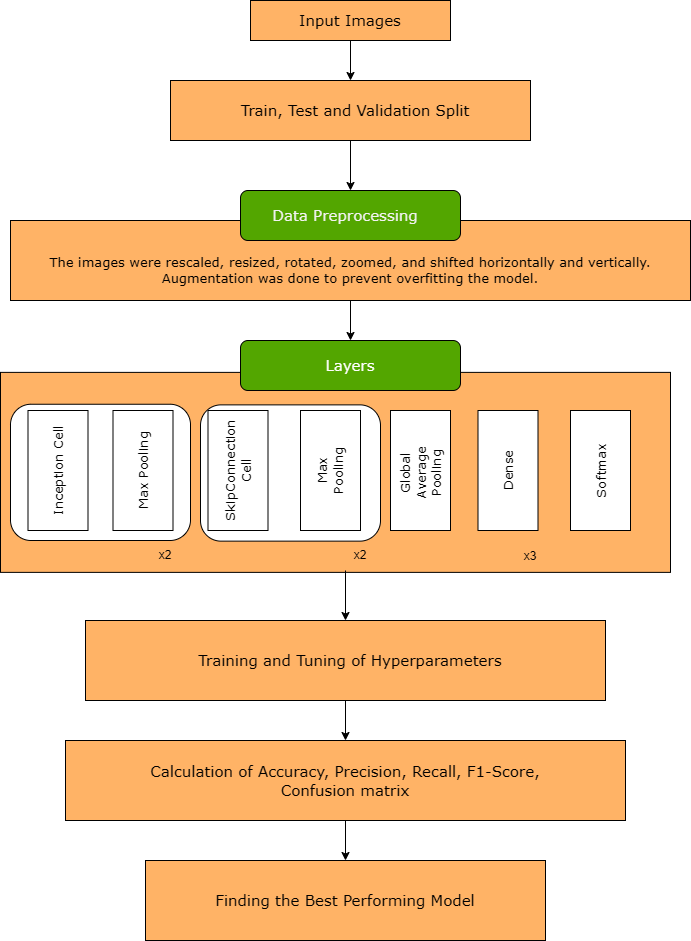
\includegraphics[width=0.94\textwidth]{preprocessing_pipeline.png}}{\fbox{Preprocessing figure: place preprocessing\_pipeline.png in paper\_figures/}}
\caption{Preprocessing and augmentation workflow. Routine preprocessing and experimental augmentation are shown as separate stages.}
\label{fig:preprocess}
\end{figure*}

\subsection{PlantDiseaseNet-Hybrid architecture}
The supplied final model accepts $256\times256\times3$ RGB input and contains two Inception-style blocks, two skip-connection blocks, four max-pooling operations, global average pooling, and a two-layer dense classifier.

\begin{figure*}[t]
\centering
\IfFileExists{paper_figures/overall_architecture.png}{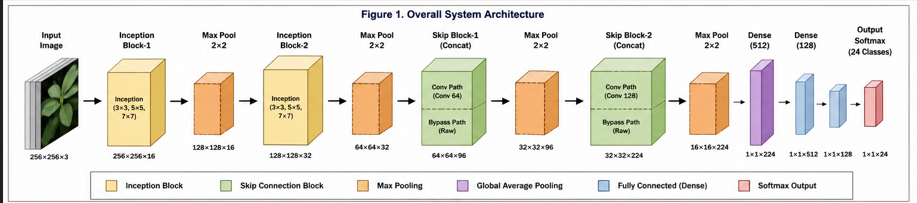
\includegraphics[width=0.96\textwidth]{overall_architecture.png}}{\fbox{Overall architecture figure: place overall\_architecture.png in paper\_figures/}}
\caption{Overall PlantDiseaseNet-Hybrid architecture.}
\label{fig:overall}
\end{figure*}

\subsubsection{Inception(Add) block}
Each block applies $3\times3$, $5\times5$, and $7\times7$ convolutions with equal branch depth. The branch outputs are fused as
\begin{equation}
Y=F_{3\times3}(X)+F_{5\times5}(X)+F_{7\times7}(X).
\label{eq:add}
\end{equation}

The design controls channel growth. Concatenating three equally wide branches would triple the branch depth, whereas addition retains the branch depth. This reduces tensor width and memory pressure while still allowing responses at three receptive-field scales to contribute to a shared representation.

\begin{figure*}[t]
\centering
\IfFileExists{paper_figures/inception_block.jpg}{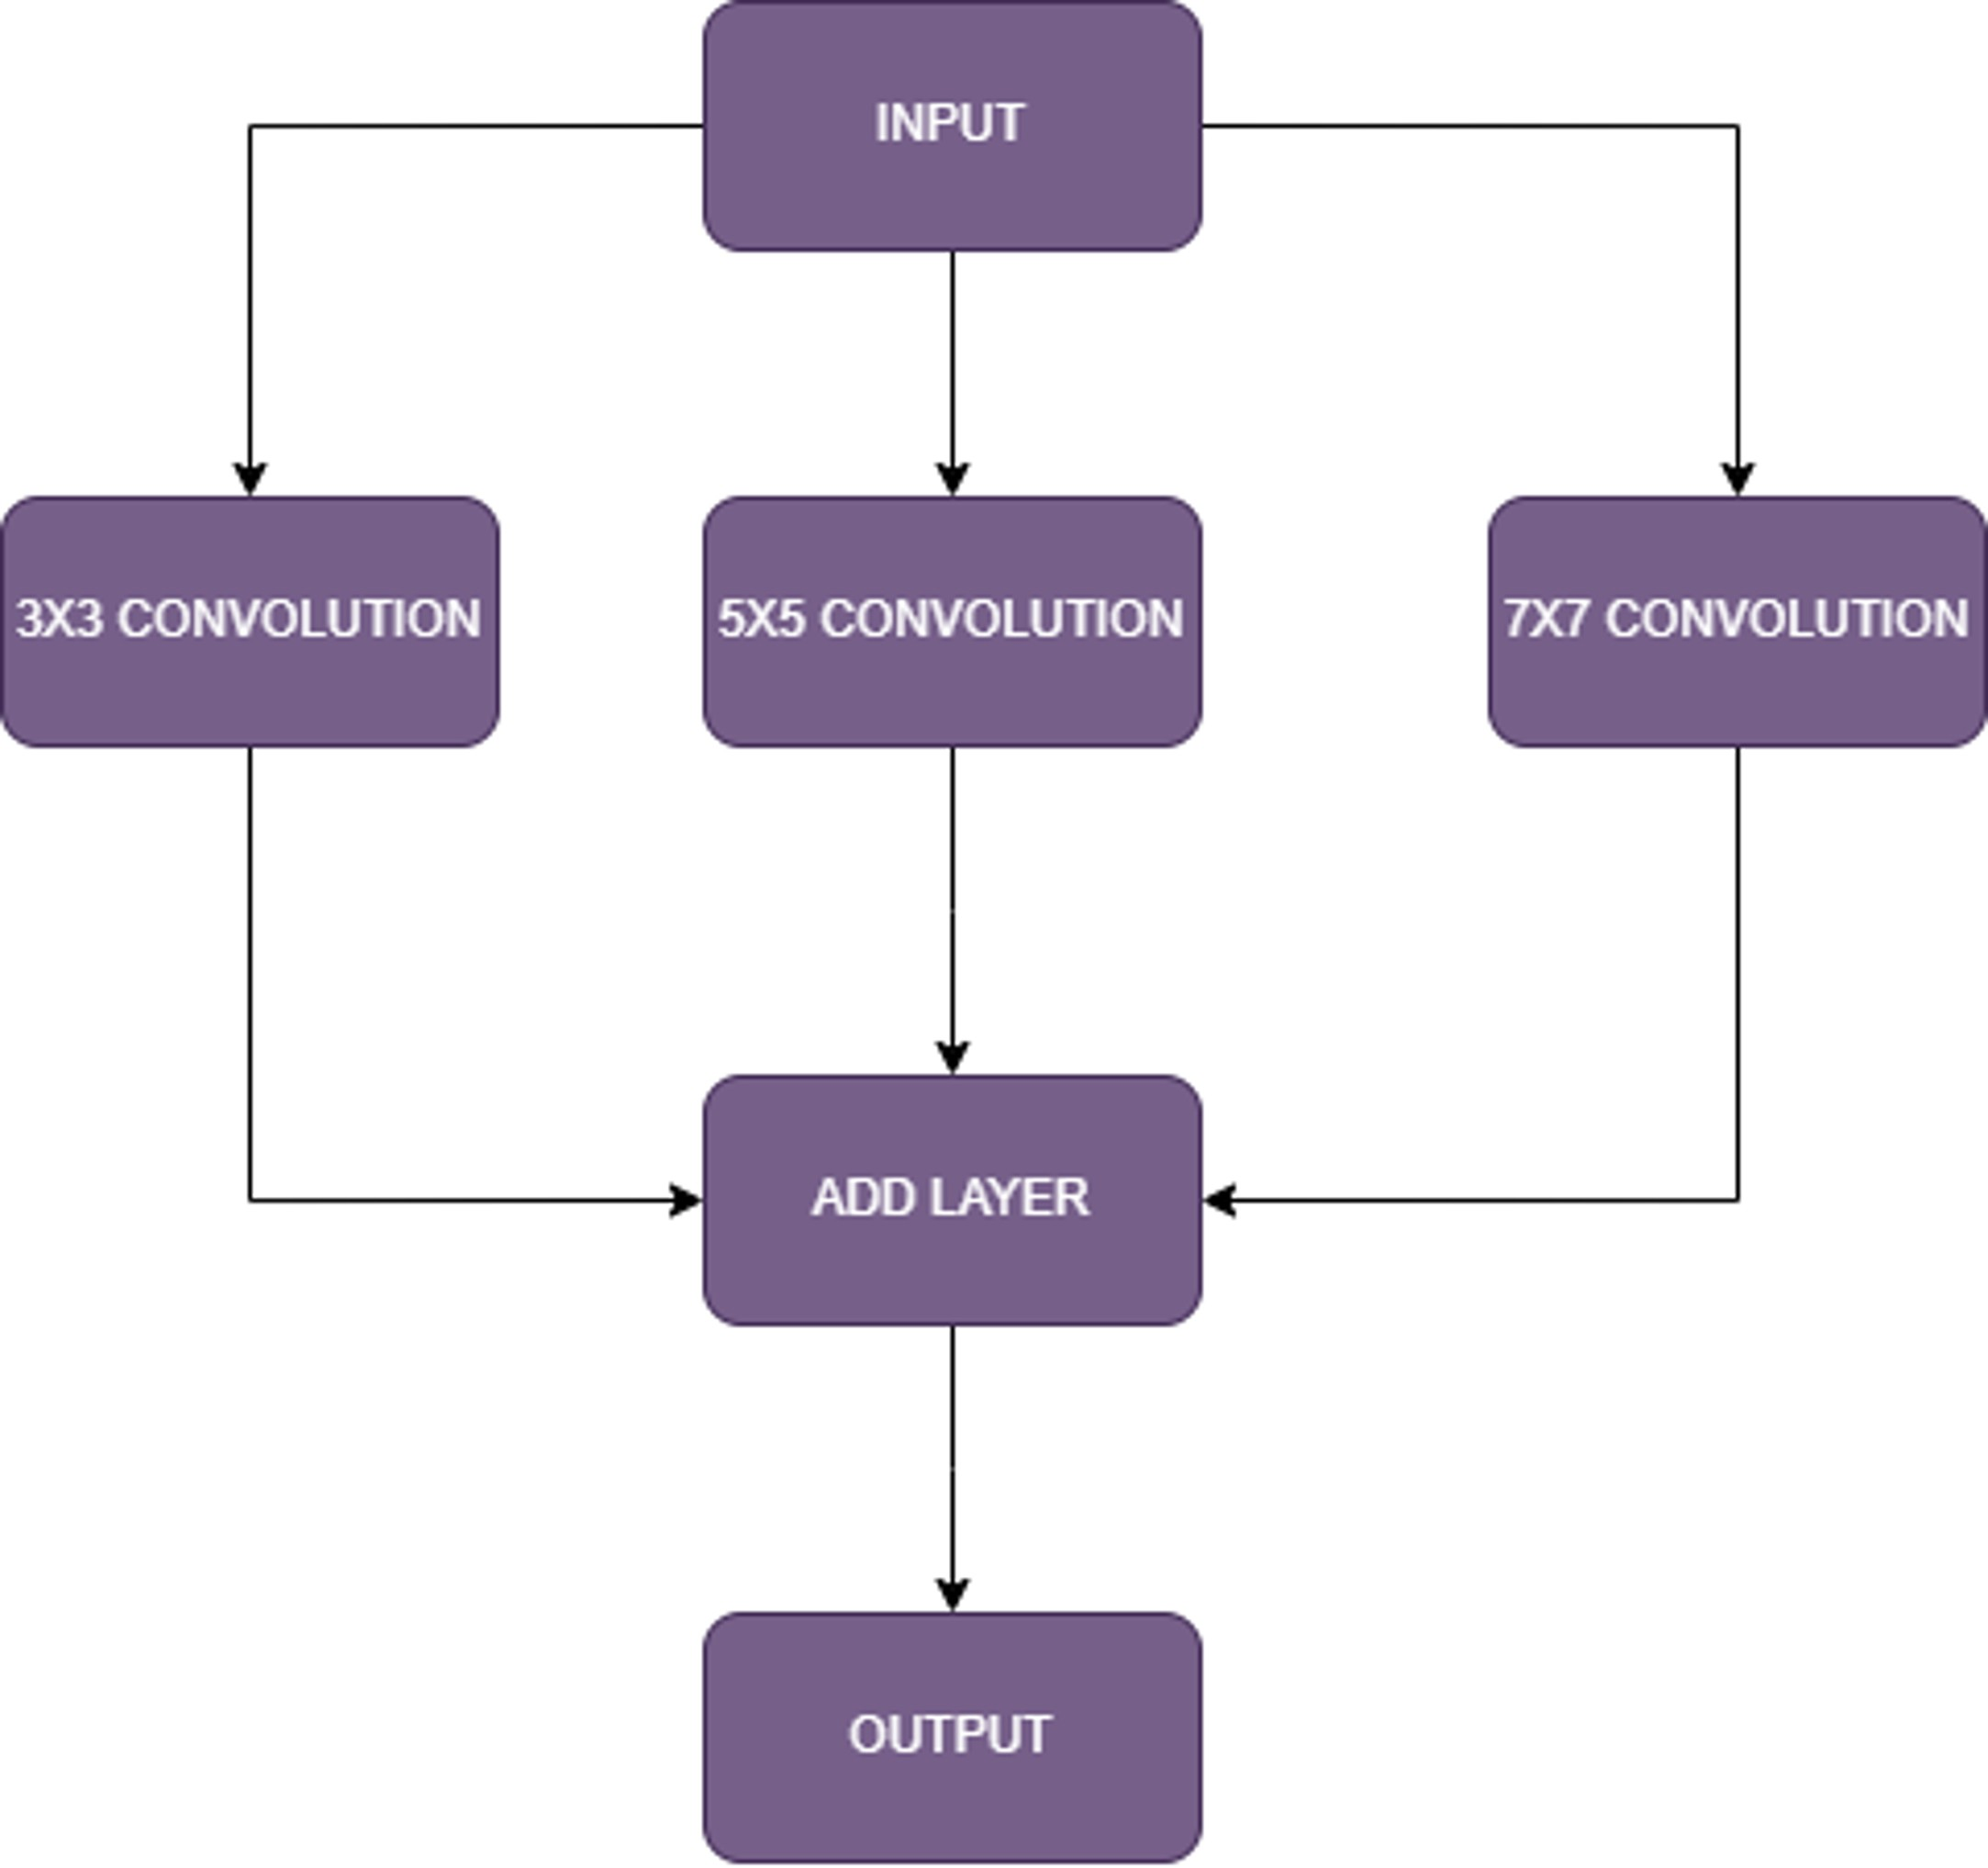
\includegraphics[width=0.68\textwidth]{inception_block.jpg}}{\fbox{Inception block figure: place inception\_block.jpg in paper\_figures/}}
\caption{Proposed Inception(Add) block.}
\label{fig:inception}
\end{figure*}

\subsubsection{SkipConnection(Concat) block}
The skip block applies a $7\times7$ convolution followed by batch normalization and concatenates the result with its input:
\begin{equation}
Y=\operatorname{Concat}(X,F(X)).
\label{eq:concat}
\end{equation}

This operation retains the earlier representation explicitly while adding newly learned features. The motivation is feature preservation and reuse, particularly when earlier layers contain spatial details that may be useful for distinguishing visually similar disease symptoms.

\begin{figure*}[t]
\centering
\IfFileExists{paper_figures/skip_block.jpg}{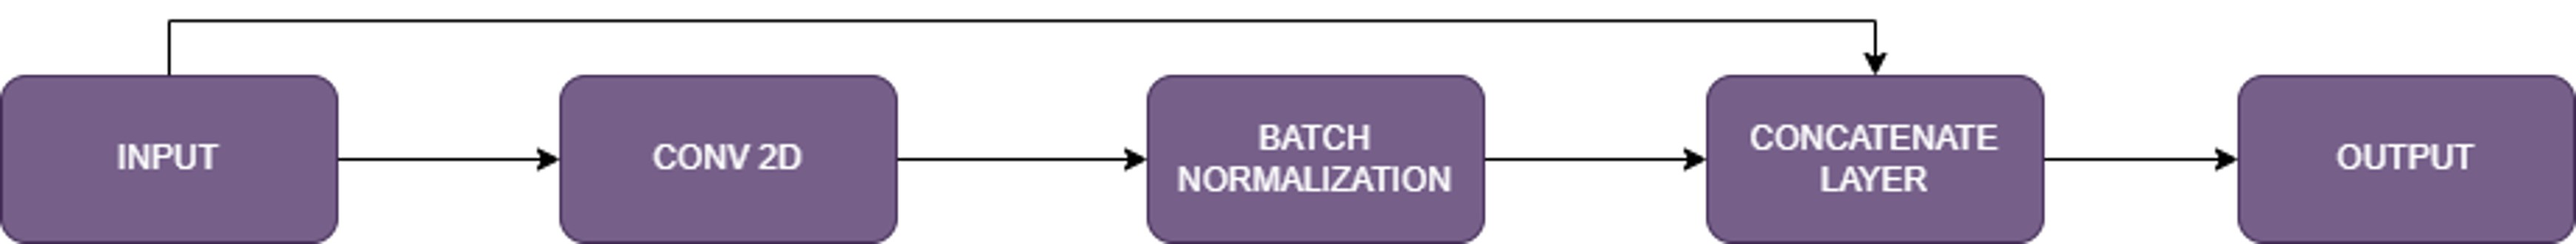
\includegraphics[width=0.68\textwidth]{skip_block.jpg}}{\fbox{Skip block figure: place skip\_block.jpg in paper\_figures/}}
\caption{Proposed SkipConnection(Concat) block.}
\label{fig:skip}
\end{figure*}

\subsection{Architecture specification}
\begin{table*}[t]
\centering
\caption{Layer-wise specification of the supplied PlantDiseaseNet-Hybrid definition.}
\label{tab:architecture}
\small
\begin{tabularx}{\textwidth}{@{}l l r X@{}}
\toprule
Layer & Output shape & Parameters & Operation \\
\midrule
Input & $256\times256\times3$ & 0 & RGB input \\
Inception Block-1 & $256\times256\times16$ & 4,032 & Three-scale additive fusion \\
BatchNorm + Pool-1 & $128\times128\times16$ & 64 & Normalisation and downsampling \\
Inception Block-2 & $128\times128\times32$ & 42,592 & Three-scale additive fusion \\
BatchNorm + Pool-2 & $64\times64\times32$ & 128 & Normalisation and downsampling \\
Skip Block-1 & $64\times64\times96$ & 100,672 & $7\times7$ convolution, BN, concatenation \\
Pool-3 & $32\times32\times96$ & 0 & Downsampling \\
Skip Block-2 & $32\times32\times224$ & 602,752 & $7\times7$ convolution, BN, concatenation \\
Pool-4 + GAP & 224 & 0 & Spatial aggregation \\
Dense 512 + Dropout & 512 & 115,200 & Classifier representation \\
Dense 128 + Dropout & 128 & 65,664 & Compact classifier representation \\
Output & 24 & 3,096 & Softmax \\
\midrule
\multicolumn{2}{r}{Total} & \textbf{934,200} & Sum of supplied Keras summary counts \\
\bottomrule
\end{tabularx}
\end{table*}

\subsection{Training configuration}
The original study configuration specifies Adam optimisation with an initial learning rate of $10^{-3}$, batch size 32, a maximum of 60 epochs, categorical cross-entropy loss, cosine warmup annealing, and early stopping with patience 12. Historical notebooks contain other configurations; therefore, the final manuscript must associate each numerical result with the configuration of its exact source run.

\begin{table}[t]
\centering
\caption{Target training configuration from the original study.}
\label{tab:hyper}
\small
\begin{tabular}{@{}ll@{}}
\toprule
Setting & Value \\
\midrule
Input size & $256\times256\times3$ \\
Batch size & 32 \\
Maximum epochs & 60 \\
Optimizer & Adam \\
Initial learning rate & 0.001 \\
Scheduler & Cosine warmup annealing \\
Early stopping patience & 12 \\
Loss & Categorical cross-entropy \\
\bottomrule
\end{tabular}
\end{table}

\subsection{Evaluation metrics}
Accuracy, macro precision, macro recall, macro F1-score, and specificity are used for aggregate evaluation. Macro averaging is retained where appropriate because it gives each class equal weight. ROC/AUC, precision--recall curves, confusion matrices, and per-class metrics are used when the matching result artifacts are available.

\section{Experimental Design}
\subsection{Primary crop experiments}
The primary experiments retain the original naming: \texttt{NB1\_Wheat\_Hybrid}, \texttt{NB2\_Cotton\_Hybrid}, and \texttt{NB3\_PlantVillage\_Hybrid}. They establish crop-specific behaviour before the combined 24-class study.

\subsection{Combined dataset and architecture study}
The original comparison contains Standard Inception, ResNet-style residual fusion, Inception with Add fusion, and SkipConnection with Concat fusion. Dataset changes themselves are not called ablations. Architectural ablation means replacing or removing a component while keeping the experimental setting sufficiently controlled. Thus the combined-dataset architecture comparison is the appropriate location for ablation claims.

\subsection{SoyDisease study}
SoyDisease is retained as a separate crop study. The executed baseline records 1,176 images across six classes: Healthy (288), Vein Necrosis (138), Dry Leaf (230), Septoria Brown Spot (284), Root Images (10), and Bacterial Leaf Blight (226). The scholarly dataset source is Kotwal et al. \citep{kotwal2024}. The improved notebook documents strategic per-class augmentation, L2 regularisation, and early stopping, but its recorded execution contains a download/extraction error; its final performance is therefore not numerically reported until a complete executed result is identified. \texttt{NB\_SoyCultivar200\_Proposed1.ipynb} is excluded.

\section{Results and Discussion}
\subsection{Verified results}
The values below are copied from committed metric files. They supersede older draft values where those values cannot be traced to the same artifacts.

\begin{table*}[t]
\centering
\caption{Verified results from committed metric artifacts.}
\label{tab:results}
\small
\begin{tabular}{@{}l l rrrrrr@{}}
\toprule
Experiment & Role & Accuracy & Precision & Recall & F1 & Specificity & Classes \\
\midrule
NB1 Wheat Hybrid & Primary & 97.81\% & 97.82\% & 97.81\% & 97.81\% & 98.54\% & 3 \\
NB2 Cotton Hybrid & Primary & 53.55\% & 53.01\% & 53.55\% & 51.66\% & 90.71\% & 6 \\
NB3 PlantVillage Hybrid & Primary & 97.67\% & 97.68\% & 97.67\% & 97.68\% & 99.83\% & 15 \\
NB4 Standard Inception & Architecture comparison & 95.33\% & 95.34\% & 95.33\% & 95.32\% & 99.80\% & 24 \\
NB5 ResNet-style & Architecture comparison & 96.04\% & 96.03\% & 96.04\% & 96.02\% & 99.83\% & 24 \\
\bottomrule
\end{tabular}
\end{table*}

The strongest verified primary results are obtained for Wheat and the selected PlantVillage experiment. The Cotton result is considerably lower and should be treated as a substantive finding rather than averaged away. Its confusion matrix and per-class report should be used to identify whether errors are concentrated in particular disease categories.

For the 24-class architecture comparison, ResNet-style fusion reaches 96.04\% compared with 95.33\% for Standard Inception in the recorded runs. This comparison does not establish superiority over the final PlantDiseaseNet-Hybrid design because complete numerical artifacts for the Inception(Add) and SkipConnection(Concat) variants have not yet been verified.

\subsection{Training behaviour and qualitative analysis}
The repository contains training curves, confusion matrices, ROC curves, per-class metrics, and class-distribution figures for the verified runs. Each figure must be paired with the notebook and metric artifact from which it was produced.

\begin{figure*}[t]
\centering
\IfFileExists{paper_figures/training_curves.png}{
\includegraphics[width=0.90\textwidth]{training_curves.png}}{\fbox{Training curves: place the matching figure in paper\_figures/}}
\caption{Training and validation curves for the selected executed experiment.}
\label{fig:training}
\end{figure*}

\begin{figure*}[t]
\centering
\IfFileExists{paper_figures/confusion_matrix.png}{
\includegraphics[width=0.72\textwidth]{confusion_matrix.png}}{\fbox{Confusion matrix: place the matching figure in paper\_figures/}}
\caption{Confusion matrix for the selected executed experiment.}
\label{fig:cm}
\end{figure*}

\begin{figure*}[t]
\centering
\IfFileExists{paper_figures/roc_curves.png}{
\includegraphics[width=0.82\textwidth]{roc_curves.png}}{\fbox{ROC curve: place the matching figure in paper\_figures/}}
\caption{ROC analysis for the selected executed experiment.}
\label{fig:roc}
\end{figure*}

\subsection{Augmentation study}
The augmentation study is presented separately from routine preprocessing. For each retained executed augmentation experiment, the final paper should show the original class distribution, the exact transformations used, post-augmentation counts, training/validation curves, and baseline-versus-augmented test metrics. The Potato augmentation notebook is excluded from the paper evidence set; it is only a presentation reference based on Mhala et al. \citep{mhalap2025}.

\subsection{Computational analysis}
The supplied final \texttt{build\_model()} summary contains 934,200 total parameters when all displayed Keras layer counts are summed. This differs from the approximately 59.8 million parameters recorded by the verified NB1--NB3 historical logs. These are not silently treated as the same model. FLOPs and inference latency must similarly be taken from a profiling artifact belonging to the exact final architecture.

\section{Limitations}
The repository contains historical notebooks with inconsistent architectures and training settings. The current evidence audit also does not yet establish complete numerical results for every augmentation and SoyDisease variant. The selected PlantVillage experiment is a subset rather than the complete 38-class PlantVillage collection. Finally, high performance on public leaf datasets should not be interpreted as proof of field deployment readiness without external field validation.

\section{Conclusion}
PlantDiseaseNet-Hybrid uses complementary fusion operations for complementary representation goals: addition controls channel growth during multi-scale extraction, while concatenation retains earlier features during deeper processing. The primary experiments and verified architecture comparisons demonstrate that performance differs materially across crop and model settings, supporting the need for systematic, dataset-specific analysis. The dedicated augmentation and SoyDisease studies are retained in the research design, but their numerical claims will be added only when their complete executed artifacts are traceable.

\section*{CRediT authorship contribution statement}
Author Name: Conceptualization, Methodology, Software, Investigation, Writing -- original draft. Anupama Arun: Supervision, Methodology, Validation, Writing -- review and editing. The authors should confirm this statement before submission.

\section*{Declaration of competing interest}
The authors declare that they have no known competing financial interests or personal relationships that could have appeared to influence the work reported in this paper.

\section*{Funding}
No external funding was received for this work.

\section*{Data availability}
The datasets are publicly available through the scholarly and dataset repositories cited in the manuscript. Publication-level sources are cited rather than relying on Kaggle pages alone.

\begin{thebibliography}{99}
\bibitem{hughes2015} D. P. Hughes, M. Salathé, An open access repository of images on plant health to enable the development of mobile disease diagnostics through machine learning and crowdsourcing, arXiv:1511.08060 (2015).
\bibitem{mohanty2016} S. P. Mohanty, D. P. Hughes, M. Salathé, Using deep learning for image-based plant disease detection, Frontiers in Plant Science 7 (2016) 1419. doi:10.3389/fpls.2016.01419.
\bibitem{szegedy2015} C. Szegedy, W. Liu, Y. Jia, P. Sermanet, S. Reed, D. Anguelov, D. Erhan, V. Vanhoucke, A. Rabinovich, Going deeper with convolutions, in: Proceedings of the IEEE Conference on Computer Vision and Pattern Recognition, 2015, pp. 1--9. doi:10.1109/CVPR.2015.7298594.
\bibitem{huang2017} G. Huang, Z. Liu, L. van der Maaten, K. Q. Weinberger, Densely connected convolutional networks, in: Proceedings of the IEEE Conference on Computer Vision and Pattern Recognition, 2017, pp. 4700--4708.
\bibitem{he2016} K. He, X. Zhang, S. Ren, J. Sun, Deep residual learning for image recognition, in: Proceedings of the IEEE Conference on Computer Vision and Pattern Recognition, 2016, pp. 770--778. doi:10.1109/CVPR.2016.90.
\bibitem{kingma2014} D. P. Kingma, J. Ba, Adam: A method for stochastic optimization, arXiv:1412.6980 (2014).
\bibitem{peyal2023} H. I. Peyal, M. Nahiduzzaman, M. A. H. Pramanik, M. K. Syfullah, S. M. Shahriar, A. Sultana, M. Ahsan, J. Haider, A. Khandakar, M. E. H. Chowdhury, Plant disease classifier: Detection of dual-crop diseases using lightweight 2D CNN architecture, IEEE Access 11 (2023) 110627--110643. doi:10.1109/ACCESS.2023.3320686.
\bibitem{mhalap2025} P. Mhala, A. Bilandani, S. Sharma, Enhancing crop productivity with fine-tuned deep convolution neural network for Potato leaf disease detection, Expert Systems with Applications 267 (2025) 126066. doi:10.1016/j.eswa.2024.126066.
\bibitem{wheatvit2022} A deep learning based approach for automated plant disease classification using vision transformer, 2022. The study documents the three-class Wheat Disease Detection dataset and its public source.
\bibitem{cotton2024} Advanced deep transfer learning techniques for efficient detection of cotton plant diseases, Frontiers in Plant Science (2024). The study documents the Cotton Plant Disease database and its six classes.
\bibitem{kotwal2024} J. Kotwal, R. Kashyap, M. S. Pathan, An India soyabean dataset for identification and classification of diseases using computer-vision algorithms, Data in Brief 53 (2024) 110216. doi:10.1016/j.dib.2024.110216.
\end{thebibliography}
\end{document}
